\chapter{Particle Reconstruction}
\label{sec:reco}

\section{The Tasks}

Our first problem, particle reconstruction, is a crucial part of any high-energy physics analysis. Here, we investigate an end-to-end ML model based on computer vision techniques, where we treat the calorimeter shower as a 3D image. Using a combined architecture, we simultaneously perform particle identification and energy measurement.

When dealing with particle reconstruction, one is interested in identifying a particle's type (electron, photon, etc.) and its momentum. An end-to-end application aiming to provide a full reconstruction of a given particle should thus be able to simultaneously solve a multi-class classification problem and a regression problem. In our study, we filter the REC dataset to make the classification task non-trivial, as described in Section~\ref{sec:data}. Since differentiating charged and uncharged particles is trivial, we judged the classification of our model on its ability to distinguish electrons from charged pions, and photons from neutral pions.

Our reconstruction networks were thus given the following three tasks:
\begin{itemize}
\item {\bf Identify electrons over a background of charged pions}: Charged pions are the most abundant particles produced in LHC collisions. They are typically located in jets, which are collimated sprays resulting from the showering and hadronization processes of quarks and gluons. On the other hand, electrons are rarely produced, and their presence is typically an indication of an interesting event occurring in the collision. A good electron identification algorithm should aim at misidentifying at most 1 in 10,000 pions as an electron. In order to increase the difficulty of our ML problem and to approach the kind of task that one faces at the LHC, we apply the HCAL/ECAL energy ratio cut as described in Section~\ref{sec:data}.
\item {\bf Identify photons over a background of neutral pions}: At particle colliders, the main background to photon identification comes from neutral pions decaying to photon pairs. In general, a generic $\gamma/\pi^0$ classification task is relatively easy, since the presence of two nearby clusters is a clear signature of $\pi^0$. Thus, we focus on events with high $\pi^0$ momentum, using the opening angle selection described in Section~\ref{sec:data}.
\item {\bf Energy measurement}: Once the particle is identified, it is very important to accurately determine its energy (and by extension, its momentum), since this allows physicists to calculate all the relevant high-level features, such as the mass of new particles that generated the detected particles when decaying. In this study, we address this problem on the same dataset used for the classification tasks, restricting the focus to range of energies from 2 to 500 GeV, and at various incident angles ($\eta$). Regression results using various neural network architectures were compared with results from linear regression, comparing both resolution and bias. The models we consider are designed to return the full particle momentum (energy, $\eta$, and $\phi$) of the incoming particle momentum. At this stage, this functionality is not fully exploited and only the energy determination is considered. An extension of our work to include the determination of $\eta$ and $\phi$ could be the matter of future studies.
\end{itemize}

\section{Baselines}

\subsection*{Classification Baseline}\label{app:BDT}

Boosted decision trees were chosen as the baseline of comparison for our classification task, due to their popularity in HEP experiments. Decision trees are effective in producing optimal cut-based decisions based on input features. A BDT is able to increase classification accuracy and stability by aggregating the results from multiple trees. Since a BDT optimizes cut selections, but still depends on the use of traditional pre-calculated features, we are able to use the BDT as a stand-in for standard HEP algorithms using feature-based cuts.

The features we use in our baseline BDT classification model~\cite{NIPS} are ones commonly used to characterize particle showers. One additional feature we added is R9, which measures the largest fraction of energy contained within a 3x3 window in a z-axis projection of the shower. This quantity provides a measure of the "concentration" of a shower within a small region. For values near 1, the shower is highly collimated within a single region, as in electromagnetic showers. Smaller values are typical of more spread out showers, as for hadronic and multi-prong showers. A comparison of R9 values between photons and neutral pions can be seen in Figure~\ref{fig:R9}, with examples of events with different R9 values being shown in Figure~\ref{fig:R9_examples}. After training, the discriminating power of various features can be seen in Figure~\ref{fig:BDT_ranking}.

\begin{figure}[htbp]
\centering
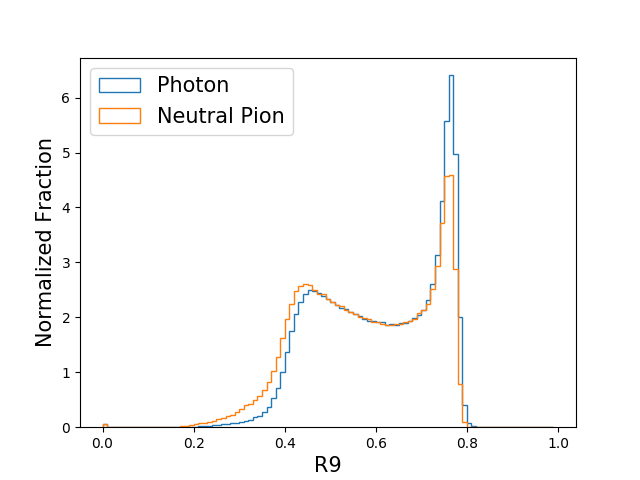
\includegraphics[width=0.6\textwidth]{Images/Calo/R9_ratios.png}
\caption{Comparison of R9 distributions between photon and neutral pion events. Photons tend to have more centralized energy depositions.
\label{fig:R9}}
\end{figure}

\begin{figure}[htbp]
\centering
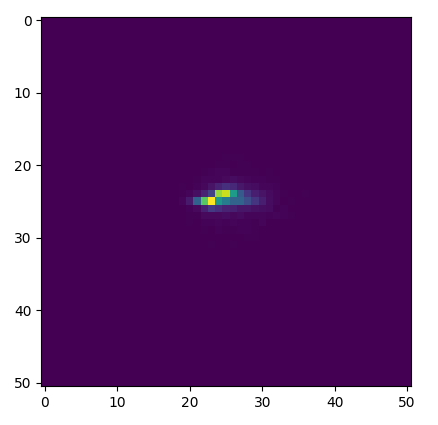
\includegraphics[width=0.4\textwidth]{Images/Calo/R9_0p42.png}
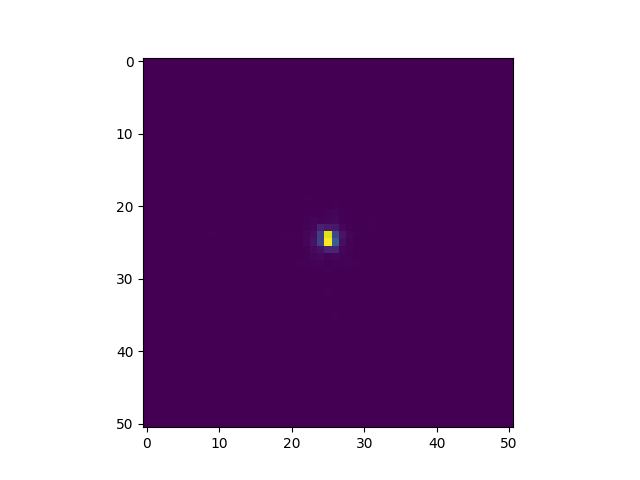
\includegraphics[width=0.4\textwidth]{Images/Calo/R9_0p75.png}
\caption{(Left) (x,y) projection of an event with R9=0.42. (Right) (x,y) projection of an event with R9=0.75.}
\label{fig:R9_examples}
\end{figure}

\begin{figure}[htbp]
\centering
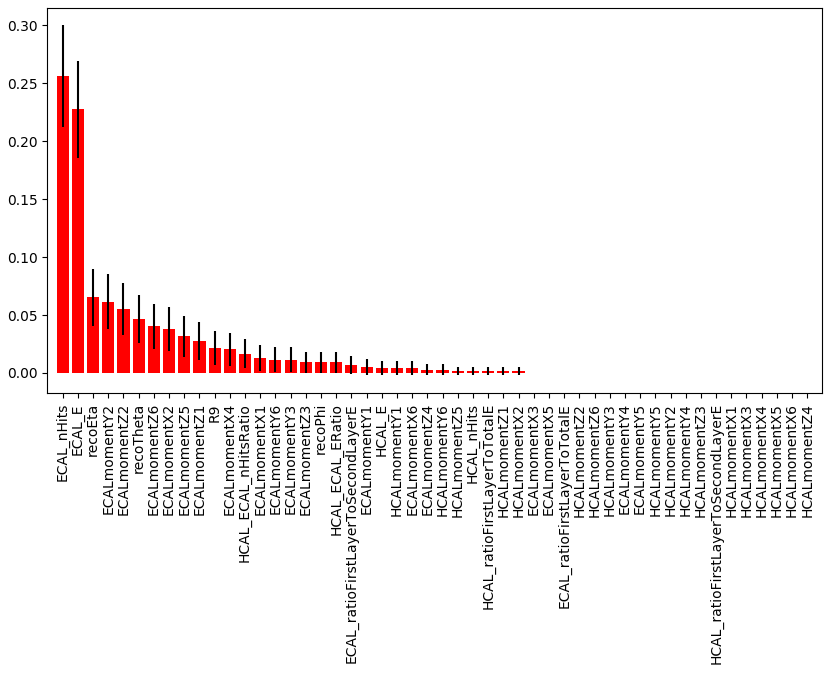
\includegraphics[width=0.7\textwidth]{Images/Calo/BDT_ranking_fixed.png}
\caption{Feature importances for inputs used in BDT training. Values shown are gini importances~\cite{Breiman}.\label{fig:BDT_ranking}}
\end{figure}

\subsection*{Energy Measurement Baseline}\label{app:regression_baseline}

We use linear regression as one of our energy measurement baselines, using ECAL and HCAL total energy as inputs, and where $a$, $b$, and $c$ are trained parameters:

\begin{equation}
E = a \cdot E_{ECAL} + b \cdot E_{HCAL} + c
\label{eq:linreg}
\end{equation}

We also investigated the use of BDTs for energy regression. This application has seen use in some LHC experiments (e.g., to study $H \rightarrow \gamma\gamma$ decays).  We used the XGBoost package in Python, with the following hyperparameters:

\begin{itemize}
\item maximum 1000 iterations, with early stopping if loss doesn't improve on the test set in 10 iterations
\item maximum tree depth of 3
\item minimum child weight of 1 (default)
\item learning rate $\eta = 0.3$ (default)
\end{itemize}

We used the following input features, as we found they gave good performance for electrons, photons, and \pizero. Adding the mean $z$ coordinate to the ECAL and HCAL total energies improved the energy resolution for all energy values, but in particular at high energy, as can be seen in Figure~\ref{fig:reg_xgb_ecalmoms}.

\begin{itemize}
\item total ECAL energy
\item total HCAL energy
\item mean $z$ coordinate of the ECAL shower
\end{itemize}

For \chpi, adding the following variables further improved the results:

\begin{itemize}
\item RMS in the $z$ direction of the ECAL shower
\item RMS in the $(x,y)$ plane of the HCAL shower
\item mean $z$ coordinate of the HCAL shower
\end{itemize}

In addition, for \chpi, around 0.5\% of events were found to have almost no reconstructed energy in the selected calorimeter window.  Including these events adversely affected the algorithm training, so they were removed for all the results shown in this and the following sections. Specifically, the raw ECAL+HCAL energy is required to be at least 30\% of the true generated energy.

The results of the XGBoost baseline are compared against linear regression in Figure~\ref{fig:reg_xgb_linreg}. The performance of XGBoost on electrons, photons, and \pizero\ is similar, achieving relative resolutions of about 6--8\% at the lowest energies and 1.0--1.1\% at the highest energies.  Compared to the baseline linear regression, the resolution improves by a factor of about two at low energy and three to four at high energy.  For \chpi, the resolution after XGBoost regression ranges between 20 and 5.4\%, with a relative improvement over linear regression of up to 40\% at high energy.

\begin{figure}[htbp]
\centering
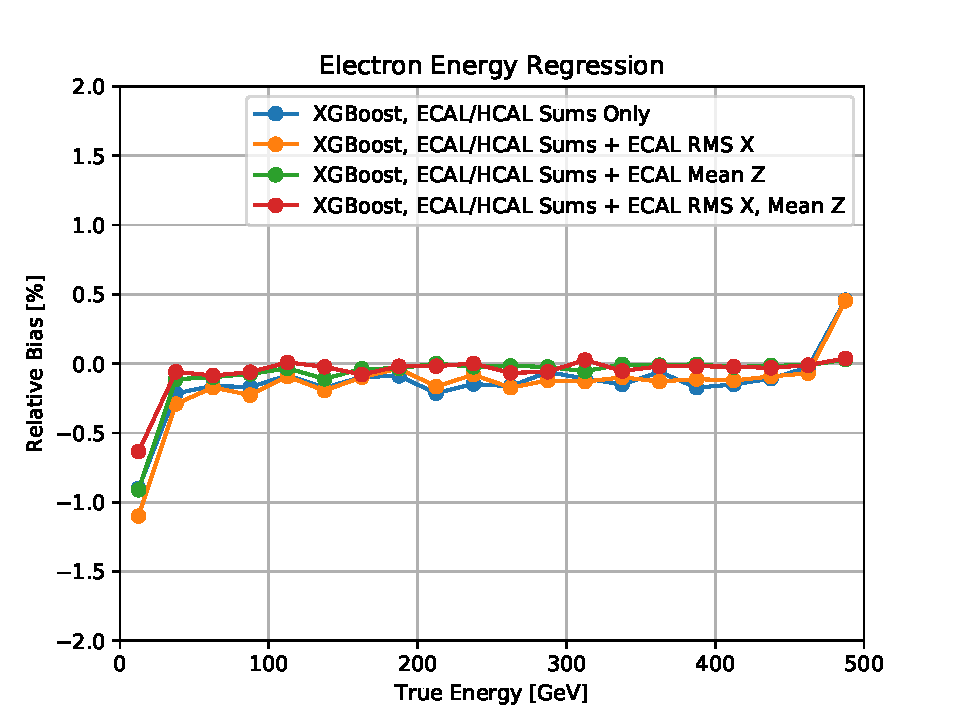
\includegraphics[width=0.45\textwidth]{Images/Calo/bias_vs_E_EleFixed_xgb_ecalmoms_zoom.pdf}
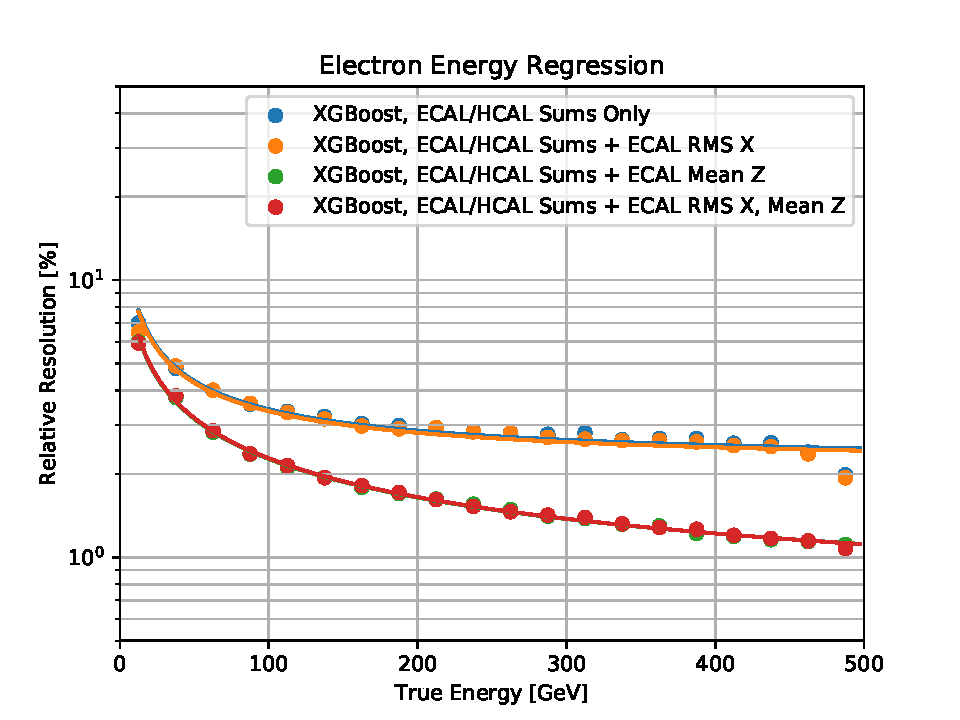
\includegraphics[width=0.45\textwidth]{Images/Calo/res_vs_E_EleFixed_xgb_ecalmoms_fits.pdf}
\caption{Bias (left) and resolution (right) as a function of true energy for the XGBoost regression predictions of particle energy, using different input features for electrons.\label{fig:reg_xgb_ecalmoms}}
\end{figure}

\begin{figure}[htbp]
\centering
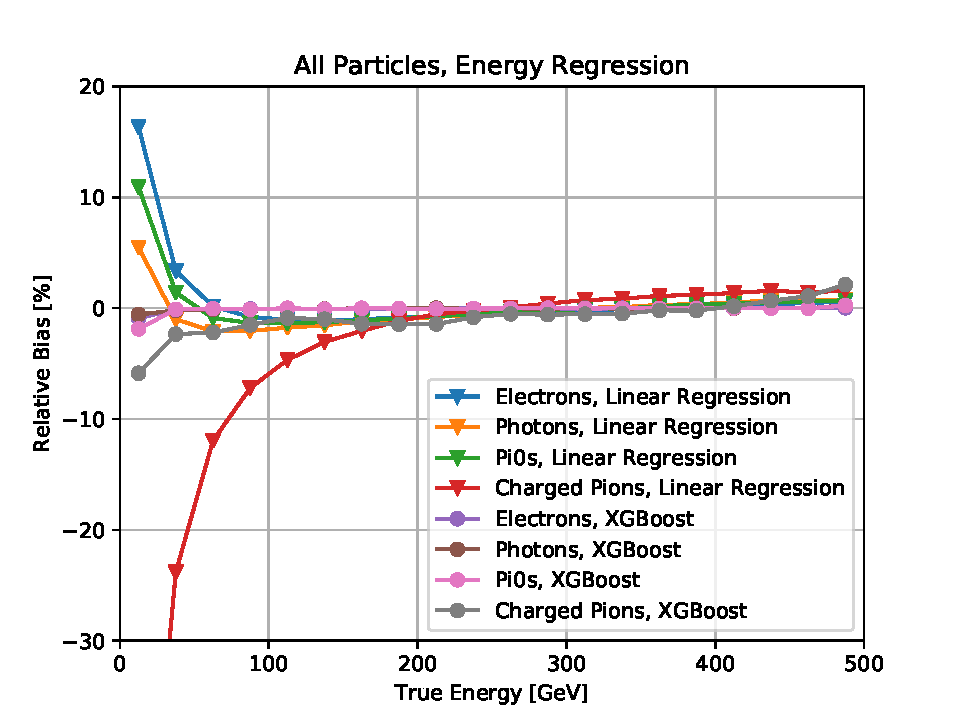
\includegraphics[width=0.45\textwidth]{Images/Calo/bias_vs_E_allparts_linreg_xgb.pdf}
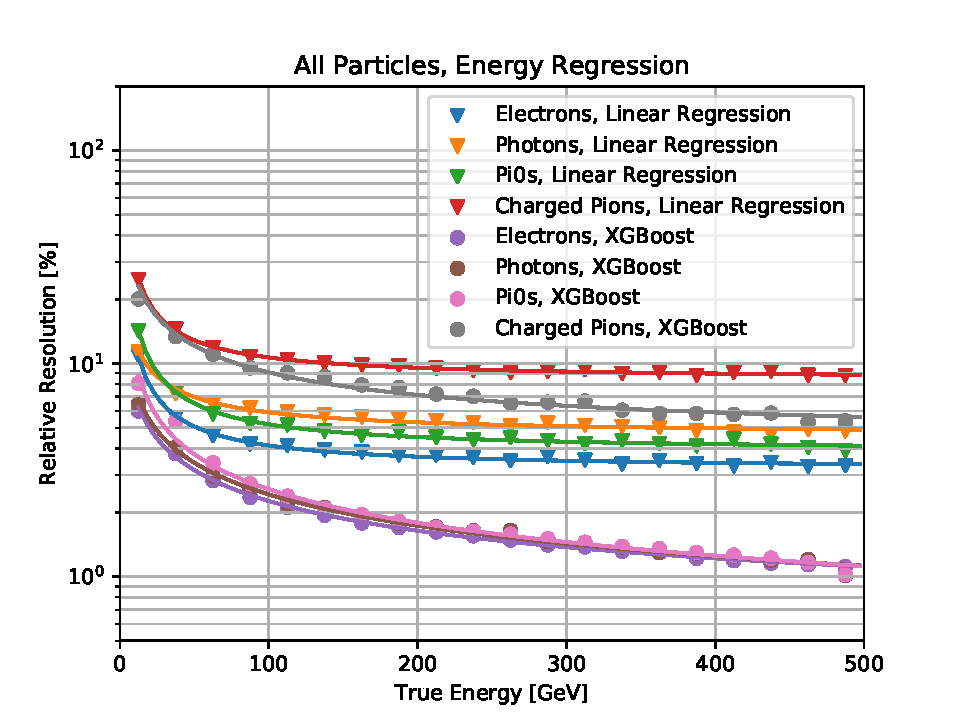
\includegraphics[width=0.45\textwidth]{Images/Calo/res_vs_E_allparts_linreg_xgb_fits.pdf}
\caption{Bias (left) and resolution (right) as a function of true energy for linear regression and XGBoost  predictions of particle energy for the different particle types.\label{fig:reg_xgb_linreg}}
\end{figure}

One drawback of using a BDT algorithm in a real-world setting is that it can not be used for energy values outside the range of the training set. That is, most tree algorithms do not perform extrapolation. This is an inherent disadvantage of the BDT when compared with the neural networks we present in this paper. However, despite this drawback, we use BDT results as a second baseline for comparison in our energy measurement task.